\documentclass{sigplanconf}

\usepackage{lgrind}
\usepackage[dvips]{graphicx}
\usepackage{verbatim}
\pagestyle{plain}

%% This bit allows you to either specify only the files which you wish to
%% process, or `all' to process all files which you \include.
%% Krishna Sethuraman (1990).

\typein [\files]{Enter file names to process, (chap1,chap2 ...), or `all' to
process all files:}
\def\all{all}
\ifx\files\all \typeout{Including all files.} \else \typeout{Including only \files.} \includeonly{\files} \fi

\begin{document}

% -*-latex-*-

\title{Linear State-Space Analysis and Optimization of StreamIt Programs}

\author{Sitij Agrawal}
\department{Department of Electrical Engineering and Computer Science}
% If the thesis is for two degrees simultaneously, list them both
% separated by \and like this:
% \degree{Doctor of Philosophy \and Master of Science}
\degree{Master of Engineering in Computer Science and Engineering}
\degreemonth{August}
\degreeyear{2004}
\thesisdate{August 26, 2004}

%% By default, the thesis will be copyrighted to MIT.  If you need to copyright
%% the thesis to yourself, just specify the `vi' documentclass option.  If for
%% some reason you want to exactly specify the copyright notice text, you can
%% use the \copyrightnoticetext command.
%\copyrightnoticetext{\copyright IBM, 1990.  Do not open till Xmas.}

% If there is more than one supervisor, use the \supervisor command
% once for each.
\supervisor{Saman Amarasinghe}{Associate Professor}

% This is the department committee chairman, not the thesis committee
% chairman.  You should replace this with your Department's Committee
% Chairman.
\chairman{Arthur C. Smith}{Chairman, Department Committee on Graduate Students}

% Make the titlepage based on the above information.  If you need
% something special and can't use the standard form, you can specify
% the exact text of the titlepage yourself.  Put it in a titlepage
% environment and leave blank lines where you want vertical space.
% The spaces will be adjusted to fill the entire page.  The dotted
% lines for the signatures are made with the \signature command.
\maketitle

% The abstractpage environment sets up everything on the page except
% the text itself.  The title and other header material are put at the
% top of the page, and the supervisors are listed at the bottom.  A
% new page is begun both before and after.  Of course, an abstract may
% be more than one page itself.  If you need more control over the
% format of the page, you can use the abstract environment, which puts
% the word "Abstract" at the beginning and single spaces its text.

%% You can either \input (*not* \include) your abstract file, or you can put
%% the text of the abstract directly between the \begin{abstractpage} and
%% \end{abstractpage} commands.

% First copy: start a new page, and save the page number.
\cleardoublepage
% Uncomment the next line if you do NOT want a page number on your
% abstract and acknowledgments pages.
% \pagestyle{empty}
\setcounter{savepage}{\thepage}
\begin{abstractpage}
Applications that are structured around some notion of a "stream"
are becoming increasingly important and widespread.  There is
evidence that streaming media applications are already consuming
most of the cycles on consumer machines \cite{Rix98}, and their
use is continuing to grow.  {\StreamIt} is a language and compiler
specifically designed for modern stream programming.  Despite the
prevalence of these applications, there is surprisingly little
language and compiler for practical, large-scale stream
programming.  {\StreamIt} is a language and compiler specifically
designed for modern stream programming.  The {\StreamIt} langauge
holds two goals: first, to provide high-level stream abstractions
that improve programmer productivity and program robustness within
the streaming domain; second, to serve as a common machine
language for grid-based processors.  At the same time, {\StreamIt}
compiler aims to perform stream-specific optimizations to achieve
the performance of an expert programmer.  This thesis develops
several techniques for scheduling execution of {\filters} in
{\StreamIt}.  The work focuses on correctness as well as
minimizing buffering requirements and stored schedule size.

\end{abstractpage}

% Additional copy: start a new page, and reset the page number.  This way,
% the second copy of the abstract is not counted as separate pages.
% Uncomment the next 6 lines if you need two copies of the abstract
% page.
% \setcounter{page}{\thesavepage}
% \begin{abstractpage}
% Applications that are structured around some notion of a "stream"
are becoming increasingly important and widespread.  There is
evidence that streaming media applications are already consuming
most of the cycles on consumer machines \cite{Rix98}, and their
use is continuing to grow.  {\StreamIt} is a language and compiler
specifically designed for modern stream programming.  Despite the
prevalence of these applications, there is surprisingly little
language and compiler for practical, large-scale stream
programming.  {\StreamIt} is a language and compiler specifically
designed for modern stream programming.  The {\StreamIt} langauge
holds two goals: first, to provide high-level stream abstractions
that improve programmer productivity and program robustness within
the streaming domain; second, to serve as a common machine
language for grid-based processors.  At the same time, {\StreamIt}
compiler aims to perform stream-specific optimizations to achieve
the performance of an expert programmer.  This thesis develops
several techniques for scheduling execution of {\filters} in
{\StreamIt}.  The work focuses on correctness as well as
minimizing buffering requirements and stored schedule size.

% \end{abstractpage}

\cleardoublepage

\section*{Acknowledgments}

    First, I would like to thank my family for all their support throughout my college years.
I would like to thank the members of the StreamIt group - in particular Jasper Lin and David Maze - for patiently
answering all my questions and for helping me understand the StreamIt language and compiler. 
I would like to thank Andrew Lamb, whose work on linear analysis of StreamIt programs provided the foundation for 
my own work on state-space analysis. His thesis and well-constructed code were invaluable to me. Rodric Rabbah, another
member of our group, gave me excellent comments about the writing in this thesis.
I would like to thank my advisor, Saman Amarasinghe, for giving me the opportunity to work on the StreamIt project and for funding
my research. Finally, I would like to thank Bill Thies for guiding me through every step of my project. That
I was able to complete this thesis is a testament to his mentoring ability. I could not have done it without him.


%%%%%%%%%%%%%%%%%%%%%%%%%%%%%%%%%%%%%%%%%%%%%%%%%%%%%%%%%%%%%%%%%%%%%%
% -*-latex-*-

\pagestyle{plain}
%\include{contents}
\section{Introduction}

The domain of stream programs is important because it stands at the
intersection of trends in applications and architectures.  Stream
programming naturally represents applications such as audio, video,
digital signal processing, and data analysis; applications that are
increasing prevalent as computing moves towards data-centric
applications and to the mobile and embedded space.  Also, by virtue of
their structure -- a graph of independent computational nodes (termed
{\it filters}) with explicit and regular communication -- stream
programs are a natural fit for exploiting coarse-grained parallelism
suitable for multicore architectures.  The interest in streaming
applications has spawned a number of streaming languages that target
the streaming domain, including StreamIt~\cite{streamitcc},
Brook~\cite{brook04}, Cg~\cite{cg03},
SPUR~\cite{spur05samos}, Spidle~\cite{spidle03}, Lime~\cite{lime10},
and SPL~\cite{spl09}.

In a stream program, filters define an atomic execution step that
repeats for many iterations; each execution step discards a number of
data items from filter's input edge.  Often, a filter does not discard
all the data items that it read for the current execution step,
requiring these inspected (but not discarded) items for a future
iteration (or iterations) of the filter.  This type of filter is
described as performing a sliding window computation on its
input. Sliding window computations are prevalent in stream programs.
Examples of sliding window computations include FIR filters; moving
averages and differences; error correcting codes; motion estimation;
and network packet inspection.  A recent study of a large streaming
benchmark suite written in the StreamIt programming language finds
that 17 of the 30 real-world benchmarks include at least one filter
that performs a sliding window computation~\cite{streamit-suite}.


Figure~\ref{fig:fir-nopeeking} shows how to perform a sliding
window FIR filter via state carried between iterations of a filter.
This implementation is difficult for the compiler to analyze and
reason about.  Some programming languages (e.g., Brook, Lime,
StreamIt, and IBM SPL) go so far as to include idioms that directly
represent sliding window computation, allowing the programmer to
specify, for each filter, the size of the window and the number of
items discarded after an execution of the filter.
Figure~\ref{fig:fir-peeking} shows how language extensions of the
StreamIt programming language elegantly expose sliding windows for
compiler analysis and optimization.

A goal of stream programming is to directly expose to the software
layer the necessary information to enable automatic management of
coarse-grained parallelism.  Stream programs expose multiple forms of
parallelism: pipeline parallelism that exists between producers and
consumers; task parallelism that exists between pairs of filters on
parallel branches of the stream graph; and data parallelism that
exists when a filter is stateless and can thus be replicated.  Data
parallelism is the most attractive, as it provides load-balanced and
limitless parallelism (as long as input data is available).  A filter
that is stateful, and cannot be data-parallelized, becomes a limit to
parallelization scalability, as the work of that filter cannot be
divided; the most load-intensive stateful filter becomes a
bottleneck.

This paper presents a compiler framework for data-parallelizing
filters that perform sliding window computations when the properties
of the sliding window can be calculated statically.  If sliding window
filters required state, this state would represent a new
parallelization bottleneck.  Sliding windows are the bottleneck in 11
of the 17 real-world benchmarks in the StreamIt Benchmark Suite that
contain sliding windows~\cite{streamit-suite}.  For example, examining
the Channelvocoder benchmark, this state would limit scalability to 18
cores, whereas our techniques scale to at least 64 cores.

Data-parallelizing a filter is performed via a transformation termed
{\it fission} (verb form {\it fiss})~\cite{streamit-asplos}.  Fission
is the process of data-parallelizing a stateless filter by duplicating
the filter a certain number of ways, assigning duplicates to distinct
cores, and correctly distributed input data to and collecting output
data from the duplicates.  The duplicated filters are referred to as
{\it products}.  When a sliding window is present, fission is
accomplished by duplicating certain input items since they are
required by multiple products.  This duplication translates into
inter-core communication, a limiting factor for scalability when
targeting multicore architectures.

Previous approaches duplicate each input data item to all products,
with products ignoring (decimating) items that are not
needed~\cite{streamit-asplos}.  We will show that this strategy limits
scalability for multicores by requiring too much inter-core
communication.  In contrast, our strategy precisely routes each input
item to the minimal set of product filters that requires the item.
Unlike previous work, our techniques are defined on
multiple input and multiple output filters, removing the need to
introduce synchronization filters that serialize data before and
after the product filters.  

Our techniques operate on {\it static-rate} stream graphs, meaning
that the number of items produced, the number of items consumed, and
the number of items inspected by each filter can be determined
statically.  Because of this property, a steady-state schedule of
filter firings can be calculated that does not grow buffers and can be
executed indefinitely~\cite{lee87}.  Our techniques are conscious of
the spatial locality between producers and consumers.  Our framework
includes techniques that can determine when spatial locality can be
increased by altering the steady-state schedule.  When applicable, our
techniques can reduce the overall sharing (and thus inter-core
communication) requirement to below a threshold percent of the total
input communication for each sliding window filter that is
data-parallelized. 

\begin{figure}[t]
\centering
\subfigure[]{\includegraphics[width=3.3in]{figures/fir-nopeeking.pdf}\label{fig:fir-nopeeking}}
\subfigure[]{\includegraphics[width=3.3in]{figures/fir-peeking.pdf}\label{fig:fir-peeking}}
\caption[Two implementations of an FIR filter.]{\label{fig:fir-code}
  Two StreamIt implementations of an FIR filter:
   (a) the non-peeking version implemented via a
  stateful circular buffer; and (b) the peeking version. Only steady-state implementation is
  given.}
\end{figure}

The framework presented is defined on a model of computation that is
agnostic of source language.  To evaluate our techniques we have
implemented them in the context of the StreamIt compiler
infrastructure~\cite{gordon-asplos06}.  Our transformations are guided
by the parallelization management techniques presented
in~\cite{gordon-asplos06}.  We employ 3 real-world benchmarks from the
StreamIt Benchmark Suite~\cite{streamit-suite} that include sliding
window computation.  We demonstrate the effectiveness of our
techniques by comparing them to previously published techniques on 2
multicore architectures: a 16-core SMP shared-memory multicore and the
64-core distributed-memory Tilera TILE64.  We show that
our techniques are required to achieve scalable parallelization on
both architectures, achieving a 6.7x mean speedup on the 16-core SMP
and a 1.8x mean speedup on the 64-core distributed memory multicore
over a previously published technique.

\subsection{Contributions}
This paper makes the following contributions:
\begin{itemize}
  % \myitem{Motivation for Exposing Sliding Windows in Stream
  %   Languages}: Without exposing sliding windows in the language, it
  % requires heroic effort by the compiler to analyze the access patterns
  % of such a filter. Without success, the compiler will not be able to
  % data-parallelize these filters.  This will prevent robust 
  % parallelization scalability for streaming applications.

  \myitem{Generalized Fission of Sliding Window Filters}: We present a
  transformation that fisses sliding window filters with multiple
  input and multiple outputs.  The technique also supports filters
  that with multiple schedules of execution.  General fission defines
  a precise pattern of communication of input data to the products
  that can be reasoned upon by our other techniques.

  \myitem{Sharing Reduction}: We are the first to present a technique
  that decides when it is possible to decrease the amount of sharing
  between fission products by altering the steady-state of a stream
  graph, thus decreasing inter-core communication.  The technique
  reasons about all the sliding window filters of the stream graph,
  and when possible, reduces the sharing requirement to below a given
  threshold percent of the total input of the filters. 

  \myitem{Data Parallelization of Stream Graph}: We present a
  framework for data-parallelizing all of the filters of a stream
  graph employing the fission transformation on individual filters and
  applying sharing reduction when possible.  This framework optimizes
  for spatial locality and enables the compiler to automatically and
  effectively manage parallelization across varying multicore
  architectures.

  \myitem{Enable Robust Parallelization Scaling for Multicores}: For
  streaming applications with sliding window computation, previously
  published data-parallelization transformations do not scale for our
  target multicores. Our techniques enable robust parallelization
  scalability by reducing inter-core communication.  We achieve a 17x
  mean parallelization speedup for a 16-core SMP and a 62.3x mean
  parallelization speedup for the 64-core TILE64 across our benchmarks.

\end{itemize}

% \begin{figure}[t]
% \centering
% \begin{subfloat}
% \begin{minipage}[b]{0.45\textwidth}
% \eightpoint
% \begin{verbatim}
% float->float filter FIR(int N) {
%   int srcBuffer[N];
%   int srcEnd = 0; 
%   ...
%   work push 1 pop 1 {
%     srcBuffer[srcEnd] = pop();
%     float sum = 0;
%     for (int i=0; i<N; i++) {
%       sum += weights[i] * srcBuffer[(srcEnd + i + 1) % N];
%     }
%     push(sum);
%     srcEnd = (srcEnd + 1) % N;
%   }
% }
% \end{verbatim}
% \vspace{-8pt}
% \end{minipage}%
% \caption{ \label{fig:fir-nopeeking}}
% \end{subfloat}%
% \qquad
% \begin{subfloat}
% \begin{minipage}[b]{0.45\textwidth}
% \eightpoint
% \begin{verbatim}
% float->float filter FIR(int N) {
%   ...
%   work push 1 pop 1 peek N {
%     float sum = 0;
%     for (int i=0; i<N; i++) {
%       sum += weights[i] * peek(i);
%     }
%     push(sum);
%     pop();
%   }
% }
% \end{verbatim}
% \vspace{-18pt}
% \end{minipage}
% \caption{ \label{fig:fir-streamit}}
% \end{subfloat}
% \caption[Two implementations of an FIR filter.]{\label{fig:fir-code}
%   Two StreamIt implementations of an FIR filter:
%    \subref{fig:fir-nopeeking} the non-peeking version implemented via a
%   stateful circular buffer; and \subref{fig:fir-streamit} the peeking version. Only steady-state implementation is
%   given.}
% \end{figure}

\section{Multicore Streaming Layer}\label{ch:lib}

Emerging multicore architectures provides an excellent target for
streaming language compilers for a number of reasons:
\begin{itemize}
\item Individual cores are optimized for computation.
\item Limited local store capacity on a core is not a severe
limitation for streaming actors. In a stream program, actors typically
embody computation, are independent of each other, have extremely
local data-access patterns, and generally have small code sizes.
\item The availability of high-bandwidth and low-latency on-chip
communication network enables a large number of scheduling options
which would not be feasible for other targets, such as computing
clusters.
\end{itemize}

In a multicore setting, a streaming language compiler (or programmer)
must address the following challenges:
\begin{enumerate}
\item Generating code that explicitly manages data communication
  (e.g., DMA operations). Architectures that provide an asynchronous
  communication model also require pipelining the data transfers (e.g.,
  double-buffering) to increase efficieny and throughput.
\item For architectures with a finite local store on a core, the code,
  input and output buffers, and the state required by the computation
  must be tightly packaged to fit into the local memory. This
  consideration is akin to locality enhancing optimizations for
  architectures with caches.
\item Performing high-level optimizations and scheduling to achieve a
  balanced distribution of work among the cores, avoiding excess
  communication, transforming code to improve efficiency, and
  ultimately delivering high processing throughput.
\end{enumerate}

The purpose of the multicore streaming layer (MSL) is to abstract
\textsf{(1)} and provide facilities that simplify \textsf{(2)} and
\textsf{(3)}. The MSL frees a compiler or programmer from needing to
deal with the details of the architecture communication model,
allowing it to focus on exploring high-level optimization and
scheduling choices. The main goal of the MSL is to provide a generic
framework for controlling and dispatching computation to multicores
that simplifies scheduling operations. The low level details that are
specific to individual platforms are embedded in the MSL library
implementation, and hidden from the programmer or the compiler. As a
result, the MSL can provide a common platform for mapping streaming
computation to multicore and enhance portability.

\section{MSL Constructs}

There are a number of stream-oriented languages drawing from
domains such as functional, dataflow, CSP and synchronous
programming~\cite{survey97}. The MSL assumes an
architecture-independent programming language for high-performance
stream programming. It requires that the stream program presented for
execution simply consist of a dataflow graph expressing the
computation. Nodes in the graphs embody computation (e.g., actors,
filters, kernels, some encapsulated code block), and edges imply data
dependencies between input and output buffers attached to the compute
nodes. An example stream graph for an MPEG-2 decoder is shown in
Figure~\ref{fig:mpeg}. Nodes in sequence expose pipeline parallelism,
and nodes in parallel expose task (two branches of a split-join that
contain different computation) and data parallelism (branches of a
split-join that contain the same computation operate on different data).

\begin{figure}[tb]
\begin{center}
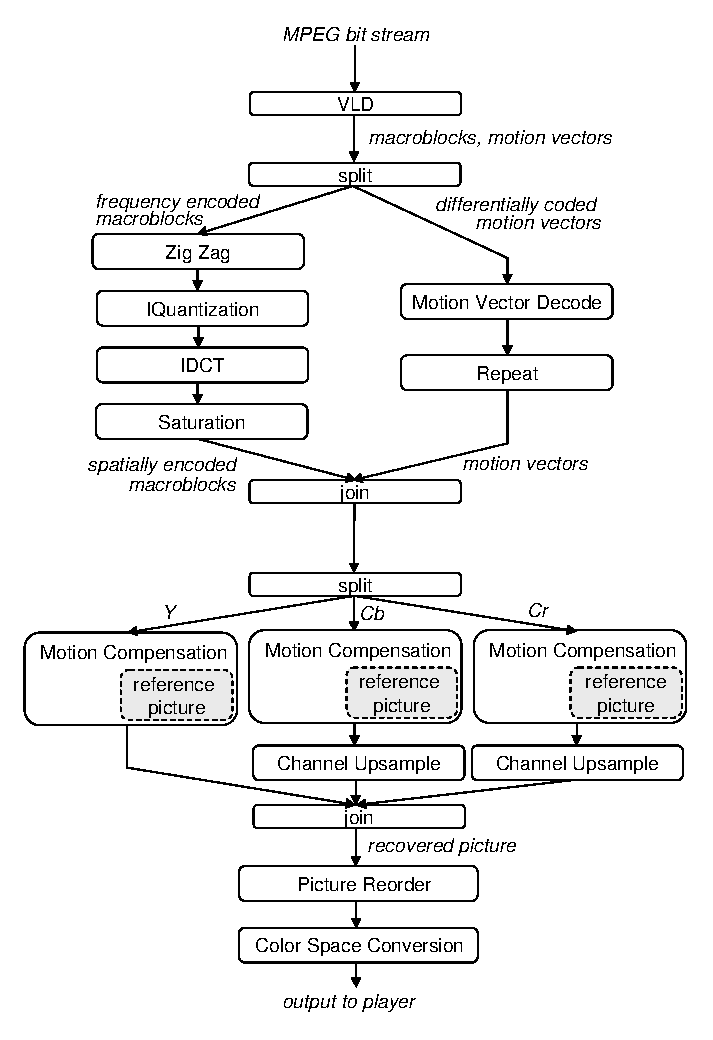
\includegraphics[scale=.70]{figs/mpeg2d}
\end{center}
\caption[MPEG-2 stream graph.]{MPEG-2 stream graph.}
\label{fig:mpeg}
\end{figure}

An execution of a stream program is an ordered sequence of node
firings. Each node follows a set of execution steps that consume a
number of items from each input channel and produce a number of items
onto each output channel.

There are two basic constructs in the MSL: \emph{filters} and
\emph{buffers}. A filter represents a generic actor that exposes a
work function which conceptually runs infinitely. Filters may be
stateful and can read from multiple input buffers and write to multiple
output buffers. While a filter can correspond directly to a
single filter in the program, a compiler can also perform
optimizations such as fusing multiple filters into a single
coarse grained MSL filter~\cite{asplos02}. Work functions are opaque to the MSL.

\emph{Buffers} are contiguous regions of data that are reserved for
temporarily storing input or output data. All buffers are circular,
and the MSL library maintains head and tail pointers for each buffer
that indicate where data begins and ends. Conceptually, a buffer has
front and back ends; data toward the front of a buffer originated
earlier in the execution of the program.

Conceptually, a filter consists of two major components, \emph{code}
and \emph{state}, as well as basic properties that describe its work
function such as the number of input and output buffers. \emph{Code}
is a single contiguous block of arbitrary data that may contain
constant data and instructions that define multiple functions; the MSL
only requires that it contain a function with a specific signature
that is used as the work function. Code for a filter is intended to be
a single modular component that can be easily relocated to different
cores. On a distributed-memory architecture where each core has a
dedicated local store (LS), code should not reference absolute
addresses (e.g., absolute branches or loads) or modify
itself\footnote{These restrictions may be ignored if it is acceptable
to not relocate filter code, or to pin the code to a single core.}.

Furthermore, code should not contain any references to mutable global
variables. Instead, code should declare and access mutable state
through fields that are local to a filter. \emph{State} contains all
mutable data that must be maintained across iterations of the work
function. Hence, state for different filters is disjoint, and filters
do not share data.

Before a filter can run on a core, it must be loaded onto the core
through the MSL library. Although the filter code and state must
reside on a core's LS while the filter work function is running, every
filter must have a permanent store location in memory. The MSL
provides facilities for loading code onto cores and copying state
between local store and memory. Note that although we refer to a
core's local store, the MSL concepts and constructs are applicable on
shared memory multicores. The locality restrictions are generally
advantageous for cache-based architectures, NUMA architectures, and
distributed-memory architectures.

A user (e.g., compiler or scheduler) provides the library with the
properties of the filter and the local store address of its work
function; the library initializes a control block that describes the
loaded filter in local store. The LS address of the control block
identifies the loaded filter in all future operations until it is
unloaded. If the filter is stateful, the library also copies its state
into local store from its permanent store in memory. Code for the
filter must be separately copied into local store through the library,
but can be located anywhere as long as the correct work function
address is provided to the library. When the user is done with a
loaded filter, it can unload the filter through the library, causing
the library to copy the filter's state back to its permanent store in
memory. Stateful filters can be loaded on at most one core at any
time, while stateless filters can be simultaneously loaded on any
number of cores (hence facilitating coarse-grained data parallelism).

This separation of code and state allows the user additional control
over how and when core local store is used. Since code is constant,
the user can preload the code of a filter onto a core even while the
filter is loaded on another core (and thus its state is owned by that
core) in preparation for loading it on the first core in the
future. If multiple (possibly stateful) filters have identical code,
only one copy of it needs to reside in memory or a core's local store
and it can be shared. When a filter is not being run, its code does
not need to be present in core local store, leaving more space free
for buffering (local store management is discussed in more detail
below).

The library provides similar facilities for allocating buffers on
cores. The size of a buffer must be a power of two, to allow
wrap-around computations to be done with a single bit-wise
\textsf{AND} instruction. Buffers are identified by the LS address
that their data region starts at in core local store; when allocating
a buffer, the library initializes a control block located immediately
before the data region that stores the buffer's head and tail pointers
and participates in data transfers. The user must specify which
buffers the filter refers to before a loaded filter can run.

%% The library does not provide memory management for core local store;
%% when filter code, filter control blocks, and buffers are allocated,
%% the user must manually specify their LS addresses and ensure that the
%% regions used by different constructs do not overlap.\footnote{The
%% library handles all resulting communication, such as copying filter
%% code and state.} This does not create as many difficulties as may
%% appear, as any memory management algorithm that can be implemented
%% internally by the library can just as easily be duplicated by the user
%% on the PPE. Moreover, allowing the user to explicitly manage local
%% store allows it to implement far more complex algorithms as
%% desired. Additionally, in this scheme, buffers and space occupied by
%% filter code and filter control blocks for stateless filters never need
%% to be explicitly deallocated -- the user can simply reuse the local
%% store region for other constructs after it is certain that they are no
%% longer in use.

Theoretically, the number of filters loaded and buffers allocated on a
core is limited only by the size of the local store.
Allocating local store is completely left to the user,
allowing a scheduler to base allocation decisions on scheduling decisions.
This is critically important on architectures like Cell that have
severely limited local store space, where the scheduler can make
much better informed allocation decisions than any other party.
%% However, there is
%% generally no useful purpose in keeping more than two filters and their
%% associated buffers on a core at any time.

%% \subsection{PPE Constructs}

%% The library does not define a filter construct for the PPE. However, because all memory is addressable by PPE code, the user can easily create similar behavior.

%% The library defines a PPE or memory buffer construct that is an extension of the core buffer. PPE buffers are not required to be circular, and buffers that are non-circular have no size limitations. PPE buffers are identified by the address of their control block, and multiple buffers can refer to the same data region, with different head and tail pointers. This is used to implement certain StreamIt features with minimal overhead, such as duplicate splitters and data-parallel execution. Because of the limited size of core local store, this functionality was considered unnecessary for core buffers.

Conceptually, data produced during the execution of a program is
contained in exactly one buffer on one core until it is consumed. The
MSL library provides facilities for moving data between buffers on
different cores.
 
\section{MSL Operations}

The MSL defines a simple set of operations to ease the mapping of stream
programs to multicores. A scheduler dispatches work items to cores by
issuing MSL commands, and is notified when cores complete
them. Each MSL command encapsulates a specific action to be
performed, and has parameters that are specified by the user. The
set of operations is divided into three main types.
\begin{itemize}
\item {\it Filter commands}: commands to load or unload filters, copy filter code into local store, attach filters to buffers, and run filters.
\item {\it Buffer commands}: commands to allocate buffers.
\item {\it Data transfer commands}: commands to move data between buffers in the local stores of different cores, or between local store and memory.
\end{itemize}

As an example, the \textsf{filter\_run} command, which runs a loaded
filter, takes two parameters: the LS address of a loaded filter's
control block and the number of times (iterations) to run the work function.
The user is responsible for ensuring that there is sufficient
data in input buffers and sufficient space in output buffers for all
specified iterations. Other commands have similar requirements. For a
complete description of all commands, see \cite{dxzhang-meng-07}.

The amount of work specified by a single command varies depending the
command parameters. Typically, work functions are small and thus
\textsf{filter\_run} commands do not take more than a few hundred
microseconds to complete; some other commands, such as allocating and
attaching buffers, are auxiliary commands and complete almost
immediately. This allows the user to quickly change scheduling
decisions and avoids tying a core into any specific long-term action.

When the user issues a command to a core, it assigns the command an ID
that must be unique among all commands previously issued to that core
that have not completed. This ID is used to notify the user when the
core finishes executing the command.

\subsection{Dependencies}

In order to keep cores supplied with work at all times, it is
necessary to limit round-trips between the scheduler and the cores
during which the cores have no commands to execute. The MSL library
provides a general facility for queuing and ordering commands on
individual cores by allowing each command to specify a set of command
IDs on the core on which it depends. Commands issued to a core are
queued and executed only after all dependencies have finished.

At any time, a command that has been issued to a core can be either
\emph{queued} (a command with unfinished dependencies), \emph{active}
(a command with all dependencies satisfied and currently being
executed), or \emph{completed} (a command for which all work has been
done, but the user has not yet been notified). From the perspective of
the user, all commands that are active on a core are run
``concurrently''. When a command is issued, all dependency IDs that
have not been issued are considered to have already completed and are
ignored.

In effect, each core maintains a small dependency graph of commands
that represents a subset in time and space of the entire
schedule. The scheduler (which may be
user code, or a dynamic scheduler running on a control processor)
continually adds commands to the dependency graph, while the core
continually processes commands that have their dependencies
satisfied. To make full use of a core, it is only necessary for the
scheduler to ensure the dependency graph on the core is never
empty. The scheduler cannot remove commands once issued, but if it
keeps the dependency graph shallow in depth, it can quickly change the
pattern of work done by a core simply by issuing a different set of
new commands.

\subsection{Command Groups}

Each command has a small amount of data associated with it, consisting
of command-specific parameters in addition to generic ID and
dependency information. Typically, the user will be issuing sets of
related commands at once. To avoid the overhead of issuing each
command individually, the user can organize commands into groups; the
library only allows entire command groups to be issued\footnote{To
issue a single command, the user can create a group containing only
that command.}. Each group specifies a sequence of commands; commands
in the group are saved and can be reissued until the group is
explicitly cleared.

Since core local store is managed by the user, the user must provide
the library with a LS address where command data will be copied to
when it issues a command group. For dependency purposes, cores treat
commands in a group as having been issued in the order they appear in
the group. 

\subsection{Scheduler Interface}

Commands issued to different cores are completely independent; the
dependency graph on each core is strictly local. The scheduler serves
as the main point of synchronization between cores by adjusting the
commands it issues to a core in response to command completion
notifications from all cores.

The scheduler is mainly callback-driven. It registers a callback
function with the MSL library that is called whenever a command issued
to a core completes. The library maintains a per-core bitmap of
command IDs that have completed; the user can query this bitmap in the
callback to determine which commands have completed and respond
accordingly. Bits in the bitmap are set until explicitly acknowledged
by the user. After an ID has been acknowledged, it can be reused for
a new command issued to the core.

%% The library does not maintain a dependency graph on the PPE. Some core
%% commands have equivalents on the PPE provided as library functions,
%% which are run immediately when called.

%% Appendix~\ref{app:ui} contains complete specifications for the interface provided by the library to user code.

\subsection{Data Transfer}

Data transfer commands indirectly result in additional points of
synchronization between cores. A data transfer conceptually moves
data from the front of a source buffer to the back of a destination
buffer, and requires two commands: a command to transfer data out of
the source buffer, issued to the core containing the source
buffer, and a command to transfer data into the destination buffer,
issued to the core containing the destination buffer. 
%% Where
%% either buffer is located in memory, the user instead calls a library
%% function.

Splitting data transfers into a pair of commands with one on each
core provides the user with explicit control over when the data
transfer occurs with respect to both cores. The library ensures
that the transfer does not occur until both commands become active on
their respective cores. The scheduler must ensure, via the
dependency graphs on cores or manually on a control processor, that
when a data transfer command becomes active on a core, the local
buffer has sufficient data or space to fulfill the transfer.

%% Data transfers impose minor alignment requirements on the buffers
%% involved due to limitations of Cell's underlying DMA model.

There are no restrictions on the size of a data transfer (except for
the size of the buffers involved), but the same size must be specified
by both commands in the pair. Each data transfer command also
specifies the address and size of the opposing buffer, since this is
information the scheduler (or user) will know in advance; however,
buffer head and tail pointers, which are more difficult to track in
advance, are handled by the library. In addition, data transfer
commands have additional inter-core requirements that the user must
ensure are met across all cores.

This ``decoupling'' of data transfers simplifies the information the
scheduler needs to keep track of. When issuing commands to one core,
it usually does not need to be concerned with the state of other
cores; as long as pairs of data transfer commands are eventually
issued with the correct parameters and dependencies, the MSL library
will automatically handle synchronization between buffers.

\subsection{Runtime Checks}

The MSL library supports a number of runtime checks that can be
enabled or disabled. When enabled, the library can validate buffer
accesses to ensure that they contain sufficient data/space, and can
perform additional checks to ensure that issued commands are
consistent. While this cannot identify all bugs in a schedule or
filter work function, it can nonetheless be very useful during the
development of a scheduler or programs. These checks can expose bugs that may otherwise appear
non-deterministically as hung executions or incorrect output.


%% \begin{figure}
%% \centering
%% \psfig{figure=beam-graph.eps,width=3.2in}
%% \caption{Stream graph of the Radar Application consisting of 12
%% channels and 4 beams. The non-linear filters are colored black. 
%% \label{fig:beam-graph}}
%% \end{figure}

\section{Illustrating Example}
\label{sec:example}

As a concrete example of space-time multiplexing, we consider the case
of a simple target detector.  As shown in
Figure~\ref{fig:target-graph}, the target detector duplicates its
input using a splitjoin; each branch of the splitjoin contains a
matched filter (to consider signals in a given range) followed by a
threshold detector.  Our analysis detects that each matched filter
computes a linear function, making it eligible for specialized code
generation in the backend.

Figure~\ref{fig:target-exec} illustrates the execution sequence that
is generated by our compiler.  Each stage in the figure shows the
computation layout for a given time partition; these stages are
executed cyclically in the steady state.  The first stage implements
the duplicate splitter by distributing the input data to distinct
off-chip DRAMs.  Each of the next four stages executes one of the
matched filters, using linear code generation to spread the
computation in a systolic fashion across the entire chip.  Finally,
the last stage executes all of the threshold filters in parallel.

In our terminology, each filter in the target detector is assigned to
its own trace.  That is, in this application, there is never a case
where two filters form a load-balanced pipeline that could execute as
a single unit on the chip.  However, the compiler recognizes the
linear filters and implements them as a 16-element pipeline that fully
utilizes the programmable on-chip network.

In the case of this example, space-time multiplexing performs 7.8X
better than a pure space-multiplexing approach~\cite{streamit-asplos}.
The cause for this dramatic speedup is that each linear trace is
executed as an independent stage.  In this form, it can utilize
template assembly code in which the operation is parallelized across
all tiles, all values are held within the registers and each cycle is
carefully accounted for.  Space-time multiplexing provides the
flexibility for such fine-grained codes to interact with general
application components.

\begin{figure}[t]
\vspace{-18pt}
\centering
\psfig{figure=target_detect.eps,width=2.5in}
\vspace{-6pt}
\caption{Stream graph for a target detector.  Linear filters are indicated in gray.
\protect\label{fig:target-graph}}
\vspace{12pt}
\psfig{figure=td_execute.eps,width=4.5in}
\vspace{-6pt}
\caption{Execution sequence for the target detector.  Each stage
indicates the mapping from filters to Raw tiles during a given time
partition.  Temporary results are buffered in off-chip DRAMs.
\protect\label{fig:target-exec}}
\vspace{-8pt}
\end{figure}

%Filters that use induction variables inherently use state to keep track of
how often it has been called through the span of the program.  We attempt 
to remove this user-facing state by introducing an iteration keyword to the 
StreamIt language.  Functionally, this iteration keyword returns how often 
the work function of the corresponding filter has been called.  Filters 
using this feature are no longer classified as stateful in the StreamIt
compiler, as the compiler has the means of fissing these filters in a 
predictable manner.

In translating higher level code into the intermediate representation, the 
iteration keyword is desugared.  The compiler adds an internal induction 
variable field for filters that use the iteration keyword.  This induction
variable is incremented at the end of each \texttt{work} call.  Any instance
of the iteration keyword is translated into a reference to this internal 
induction field.  

This desugaring process introduces induction variable state to the intermediate
representation of the filters.  Modifications must also be made to the fission 
process to allow the compiler to fiss these stateful filters and ensure 
consistency between fission products after fission.  

The fission process now modifies the fission products by adding the 
following values as fields of the products:
\begin{itemize}
	\item \texttt{start}: the value of the induction variable each product starts with.
	\item \texttt{reps}: how often the \texttt{work} function of the product is 
	  called between rounds.
	\item \texttt{total}: the sum of all reps of all fission products. This value is 
	  the same amongst all fissed products.
\end{itemize}
Accordingly, each fission product should start each round with induction values
of
\begin{center}
\texttt{total}*\texttt{n} + \texttt{start}
\end{center}
and range up to the value
\begin{center}
\texttt{total}*\texttt{n} + \texttt{start} + \texttt{reps} - 1
\end{center}
where \texttt{n} is a nonnegative integer indicating how many rounds have
been run in the span of the program.  We have to account for the off-by-one
error as the first iteration is run.

At the end of each fission product \texttt{work}, after incrementing the 
induction value, a check must be made to see if it is necessary to increment 
the induction variable to the next round of  values.  This will prevent certain
fissed products from making calls with duplicate induction values.  
\begin{center}
\texttt{iter} - \texttt{start} - \texttt{reps} \% \texttt{total} == 0
\end{center}
The fissed products must check that the current induction value less the 
\texttt{start} and \texttt{reps} of that fissed product is divisible by the 
\texttt{total}.  This is consistent with the maximum value per round as 
indicated above.  Once the fissed product's induction value has reached 
this value, it must be set to:
\begin{eqnarray*}
\texttt{iter}_{n+1} &=& \texttt{iter}_{n} + (\texttt{total} - \texttt{reps}) \\
&=& (\texttt{total}*\texttt{n} + \texttt{start} + \texttt{reps}) \\
&&  \ \ +\ (\texttt{total} - \texttt{reps}) \\
&=& (\texttt{total}*(\texttt{n+1}) + \texttt{start})
\end{eqnarray*}
which is the starting iteration value of the next round, as defined.

The scheduler may also modify the multiplicity of the rounds.  The field values
added to the fissed products must, in turn, be updated to reflect this change.
Since all fissed products will be multiplied by the same steady multiplicity
factor, we can simply multiply each of the \texttt{start}, \texttt{reps}, and 
\texttt{total} values by the same steady multiplicity value.

%\input{streamit-mapping}
\section{Scheduling Paradigms}

%% A schedule $\phi$ implies buffering requirements between actors, or in
%% other words, it imposes a minimum bound on the size of each FIFO
%% between pairs of actors. An actor cannot fire until its input channel
%% carries enough data for the phase to complete. An actor that consumes
%% a variable amount of data can be modelled as an actor that always
%% consumes a single item from its input, buffers the item internally and
%% updates its internal state. When it has buffered a sufficient quantity
%% of items of its phase to fire, it will then execute.

It is possible to devise a schedule statically (e.g.,  compile time or
at graph creationg time) or dynamically (e.g., runtime). The goal of a
scheduler is often simply to maximize the utilization of any number of
given resources. In the age of multicore architectures, a scheduler
will need to utilize the cores to increase concurrency and hence
improve the throughput of a given streaming application.
We assume a decoupled multicore architecture where each processing
core has its own local storage, and can only access data in its local
memore. The architecture provides some mechanism for moving data
between cores, or from main memory to the core. Examples of decoupled
multicores architectures are Cell~\cite{cell} and Tile64~\cite{tilera}.

A dynamic scheduler is conceptually easy to understand. The scheduler
maintains an internal representation of a given stream graph (e.g.,
list or priority queue). In a multicore architecture, when there is a
core available, the scheduler scans its interal representation of the
stream graph, and determines which actor is ready to fire; recall that
an actor is ready to execute when there is sufficient buffering on its
input channel (i.e., data dependence is satisfied).  To simplify
matters, we only consider actors where the I/O rates are known and do
not vary from one instance of a phase to the next instance of the same
phase; we will relax this constraint in later sections of the paper.

The scheduler assigns the actor to the available core. The core is
also informed where the input buffer for the actor resides in memory,
and where in memory to commit (buffer) the output of the actor for its
successors. The scheduler then updates its internal representation to
indicate the actor firings and implement a fairness policy to assure
overal progress (e.g., a roundrobin scheduler).

The dynamic scheduler essentially maximizes ulitization by pipelining
the execution of the stream graph and overlapping actor firings. For
example, consider a stream graph $A\rightarrow B$ where $\rightarrow$
denotes a FIFO connection between two actors, here $A$ and $B$. A
scheduler for a two processor multicore ($P_1$ and $P_2$) will assign
$A$ to processor $P_1$ and when $A$ completes its firing, the
scheduler assigns $B$ to processor $P_2$. While $B$ is running
however, the scheduler can determine that another firing of $A$ is
possible and hence it instructs $P_1$ to execute the actor again, and
the output is buffered such that the corresponding (i.e., second)
firing of $B$ consumes the correct data from the second instance of
$A$.

Let the expected (mean) work units required by actor $X$ to complete
running a phase be $W_X$. In the example above, when $W_A > W_B$
the processors will proceed at different rates and $P_1$ becomes a
bottleneck. To mitigate the issue, the scheduler can run multiple
instances of $A$ initially thus buffering a sufficient amount of data
and creating some slack between the two processors. This avoids
stalling the exectution and can lead to better utilization.

The are numerous heuristics and optimizations that a dynamic scheduler
can employ to orchestrate the execution of a stream graph on a
multicore. Ultimately the goals of the scheduler are to maximize
utilization and throughput, and it strives to do so by balancing the
load on the processors, maintaining adequate buffering between actors,
and trying to do so with little runtime ovearhead.

Since a dynamic scheduler is running along with the application, it
must be efficient in its orchestration of the schedule. 

There are several concerns that arise. Large stream graphs and massive
multicores present dual obstactles that limit the scalability of a
centralized dyanmic scheduler. It is possible to devise distributed or
hierarchical dynamic schedulers but that comes with additional
implementation complexity.

%% XXX more on the drawbacks

\section{Performance}\label{ch:perf}

We evaluate the performance of the MSL library and StreamIt compiler backend
on a set of four StreamIt applications and using different scheduling
methodologies. The applications are described in Table~\ref{fig:perf:apps}.
For statically-scheduled benchmarks, the scheduler executes a sufficiently
coarsened steady state to reduce library overhead, and imposes an explicit
synchronization barrier between steady state iterations. The dynamic scheduler
automatically coarsens work functions as necessary.

\begin{table}[!htb]
\begin{center}
\begin{tabular}{|l|p{2.25in}|}
\hline
BitonicSort & 8-element bitonic sort \\
\hline
DCT         & 16x16 IEEE reference DCT \\
\hline
FFT         & 256-element FFT \\
\hline
MPEG        & MPEG-2 block and motion vector decoding (subset of full MPEG-2 decoder) \\
\hline
\end{tabular}
\end{center}
\caption{Benchmark applications.}
\label{fig:perf:apps}
\end{table}

The benchmarks were run on PlayStation 3 hardware, which only provides
six usable SPEs. All benchmarks were scheduled to use six SPEs except
for the two MPEG benchmarks, which use five SPEs.
Benchmarks were run for a large number of steady state iterations
to reduce the effect of one-time execution startup overhead.
Performance results are given in Table~\ref{fig:perf:stats}.

\begin{table*}[!tb]
\begin{center}
\begin{tabular}{|l|r|r|r|r|r|r|}
\hline
                             & Util (\%) & Lib (\%) & Sched (\%) & Min Sched (\%) & Max Sched (\%) & Throughput \\
\hline
\textsf{BitonicSort\_static} & 97.1 & 0.1 &   2.9 &       2.9 &       2.9 &        0.5 GOPs \\ \hline \hline
\textsf{DCT\_static}         & 97.7 & 1.0 &   1.3 &       1.3 &       1.3 &        3.2 GFLOPs \\ \hline \hline
\textsf{FFT\_c}              & 99.1 & --- &   --- &       --- &       --- &        2.5 GFLOPs \\ \hline
\textsf{FFT\_static}         & 98.6 & 0.6 &   0.9 &       0.9 &       0.9 &        1.9 GFLOPs \\ \hline
\textsf{FFT\_dynamic}        & 88.8 & 9.2 &   2.0 &       1.2 &       2.9 &        2.2 GFLOPs \\ \hline
\textsf{FFT\_pipeline}       & 78.0 & 3.6 &  18.5 &       4.2 &      33.9 &        1.9 GFLOPs \\ \hline \hline
\textsf{MPEG\_static}        & 95.1 & 1.0 &   3.9 &       1.5 &       8.1 &       46.9 fps \\ \hline
\textsf{MPEG\_dynamic}       & 97.8 & 1.7 &   0.5 &       0.3 &       0.8 &       48.2 fps \\ \hline
\hline
\end{tabular}
\end{center}
\label{fig:perf:stats}
\caption{Benchmark performance.}
\end{table*}

The \emph{Util} column gives the average SPE utilization of the
benchmark. This is the percentage of total execution time spent inside filter work functions,
averaged over all SPEs. The remainder is overhead, which we divide into two categories:
\emph{library overhead} and \emph{scheduling overhead}. \emph{Library overhead}
is time during which an SPE has active \textsf{filter\_run} commands but is not
running a work function. This type of overhead is added entirely by library code
when it is either dispatching or executing other commands.
\emph{Scheduling overhead} is time during which an SPE has no active
\textsf{filter\_run} commands. During this time, the SPE has no useful work to do.
It may be either \emph{i}) waiting for filters to be scheduled or \emph{ii})
waiting for sufficient input or output data to be transferred to allow a scheduled filter to run
(i.e., due to inadequate double-buffering).
When large, scheduling overhead can be viewed as resulting from the scheduling algorithm
(or the nature of the program). However, a component of scheduling overhead is also
due to the latency/efficiency with which the library executes commands.

The \emph{Lib} and \emph{Sched} columns give the average library and scheduling overhead
as a percentage of total execution time, averaged over all SPEs.
The \emph{Min Sched} and \emph{Max Sched} columns give the scheduling overhead
(as a percentage of total execution time) on the SPEs with the minimum and maximum
scheduling overhead; wider ranges indicate larger work imbalance
resulting from the scheduling algorithm.
For \textsf{BitonicSort\_static}, the \emph{Throughput} column gives
billions of compare operations per second. For the MPEG benchmarks,
the \emph{Throughput} column gives the number of 352x240 frames processed per second.
For all other benchmarks, the \emph{Throughput} column gives GFLOPs.

The \textsf{BitonicSort\_static}, \textsf{DCT\_static}, and \textsf{FFT\_static} benchmarks
are statically scheduled and generated by the StreamIt compiler.
These applications are fully data-parallel and the compiler fuses the stream graph
into a single filter, which is then duplicated to the number of cores.
As expected from fully data-parallel programs, average utilization remains nearly the same
as the number of SPEs is varied from one to six and scheduling overhead is essentially identical
on all SPEs, demonstrating nearly perfectly linear speedup.
The total overhead in each benchmark is less than 3\%. Scheduling overhead appears
to dominate total overhead, largely due to the synchronization barrier after each steady state
iteration that creates repeated additional costs as the program executes.

For programs consisting of a single fused data-parallel filter, the dynamic scheduler produces identical performance as static scheduling. Results for the dynamic scheduler on these applications are not separately given.

The \textsf{FFT\_dynamic} and \textsf{FFT\_pipeline} benchmarks are different manual implementations of the FFT application. The FFT stream graph consists of a single pipeline with 15 filters. \textsf{FFT\_dynamic} schedules this pipeline using the dynamic scheduler. 

In \textsf{FFT\_pipeline}, the stream graph is first manually fused into a pipeline of six filters, each of which is statically placed on a different SPE. All communication except for input and output is done directly between SPE local stores and remains entirely on-chip. GFLOPs numbers for \textsf{FFT\_dynamic} and \textsf{FFT\_pipeline} can be compared with each other but not directly to \textsf{FFT\_static}.
The former two have manual work function implementations that are slightly more efficient than the compiler-generated code.

For \textsf{FFT\_dynamic}, scheduling overhead is low and very similar across SPEs.
This indicates that the dynamic scheduler has no difficulties keeping all SPEs supplied with work.
Moreover, the results show that
if there is sufficient memory bandwidth, as is the case with the Cell architecture, it is practical to
perform all buffering to memory, avoiding core-to-core communication entirely.
Average utilization remains nearly identical as the number of SPEs is varied from one to six,
indicating almost perfectly linear speedup.

However, the library overhead on this benchmark is high, approaching 10\%, resulting in somewhat low average utilization. This overhead has two main sources: \emph{i}) individual filters in the pipeline have much lower communication--computation ratios than the single fused filter in the \textsf{FFT\_static} benchmark; and \emph{ii}) the dynamic scheduler continually issues additional commands to switch filters between SPEs, which are not needed in a static schedule.

For \textsf{FFT\_pipeline}, a single filter/SPE in the middle of the pipeline is the bottleneck.
Although average utilization is low, it is not due to library overhead, which is low.
Average scheduling overhead is high and varies widely between SPEs:
the bottleneck SPE had 92\% utilization, while the least-utilized SPE had only 63\% utilization.
In general, this illustrates the difficulty of performing direct static SPE--SPE pipelining.
Although SPE--SPE pipelining keeps communication on-chip, where extremely high bandwidth
is available and there is no danger of exhausting comparatively limited memory bandwidth,
work imbalances between filters make it difficult to fully utilize all SPEs.

For comparison, \textsf{FFT\_c} is a hand-tuned implementation of \textsf{FFT\_static} that
does not use the MSL library. The same work function code is used as \textsf{FFT\_dynamic} and
\textsf{FFT\_pipeline} (however, this is different from \textsf{FFT\_static},
which is generated by the StreamIt compiler) and data transfers are fully double-buffered.
Compared to \textsf{FFT\_c}, \textsf{FFT\_dynamic} is approximately 12\% slower, most of which
is due to library overhead. \textsf{FFT\_pipeline} is significantly slower, but this
is entirely due to the major work imbalance it exhibits.

MPEG has a small amount of state and cannot be fused into a single filter.
The compiler fuses the stream graph down to a single stateful filter and
a single stateless filter as the branches of a two-way splitjoin.
When mapping this to the MSL library, both statically- and dynamically-scheduled benchmarks
explicitly treat the scattering and gathering operations as separate stateless filters,
resulting in four total filters to schedule.

The \textsf{MPEG\_static} benchmark statically software-pipelines the four filters.
We generated the static schedule for five SPEs by manually profiling, duplicating, and
partitioning filters, and manually generating control code to issue the resulting schedule.
The mapping of filters to SPEs in the partition that we obtained is given in
Table~\ref{fig:perf:mpegs}.

\begin{table}[!htb]
\begin{center}
\begin{tabular}{|r|l|}
\hline
SPE & Filters \\
\hline
0 & $n$ splitter, $n$ stateful \\
\hline
1 & $6n$ joiner \\
\hline
2 & $2n$ stateless \\
\hline
3 & $2n$ stateless \\
\hline
4 & $2n$ stateless \\
\hline
\end{tabular}
\end{center}
\caption{Partition for \textsf{MPEG\_static} benchmark.}
\label{fig:perf:mpegs}
\end{table}

This partition exhibits a slight work imbalance: SPE 0 has slightly less work than SPE 1,
which has slightly less work than the remaining SPEs.
As a result, there is a small variation in scheduling overhead, resulting in somewhat lower
utilization than could be achieved.
The bottleneck SPEs were 98\% utilized, while SPE 0 was 90\% utilized.
Aside from the work imbalance, which can be reduced with better partitioning,
this benchmark shows that static software pipelining using the MSL library can be done
with very low overhead.

The \textsf{MPEG\_dynamic} benchmark uses the dynamic scheduler to schedule the four filters.
As with \textsf{FFT\_dynamic}, average utilization is very similar across all SPEs,
and there is still nearly perfectly linear speedup as the number of SPEs is varied.
Compared to the static schedule, the dynamic scheduler is not limited to executing
repetitions of a steady state and does not impose any synchronization barriers.
However, in order to dynamically switch filters on cores, it must issue more commands.
This translates into slightly lower scheduling overhead but slightly higher library overhead.
Overall, the dynamic scheduler is able to more efficiently distribute work across
all available cores, resulting in higher average utilization and 2.8\% increased throughput
compared to \textsf{MPEG\_static}.

It must be noted that the throughput obtained in these benchmarks is low
compared to the maximum performance attainable on Cell and the performance of other
implementations of the same benchmarks.
No SIMD vectorization (either automatic or manual) was performed within
filter work functions for any of the benchmarks;
as a result, they did not take advantage of the SIMD capability of Cell SPEs.
In addition, filter code could have been considerably optimized. For instance,
\textsf{FFT\_static} performs more integer operations to maintain loop counters than actual FLOPs.
However, the high utilization demonstrated in the benchmarks should extend to
real-world, optimized applications as long as individual filter work functions
perform a comparable amount of work.

\mysection{Related Work}
\label{sec:related}

This paper builds directly on the work done to analyze and optimize
linear components in StreamIt graphs \cite{Lamb}. We extend the
theoretical framework for linear analysis to state space analysis in
order to apply our optimizations to a wider class of applications.
Specifically, state space analysis applies to filters with persistent
state, and feedback loops can be combined into a single state space
representation; neither of these cases are handled by linear analysis.
The extension from linear analysis to state space analysis required a
fundamental change to the underlying representation, as well as a
complete reformulation of the rules for combination and expansion.
Moreover, this paper introduces novel optimizations of state removal
and minimal parameterization, both of which operate on the state space
representation.

Several other groups are researching methods for automated DSP
optimizations. SPIRAL \cite{Spiral} is a system developed to generate
libraries of DSP transforms. These libraries are designed for specific
architectures, and can be re-optimized when hardware is upgraded or
replaced. Other such libraries that have been designed include a
package for linear algebra manipulations by the ATLAS project
\cite{Atlas} and portable high-performance FFTs (Fast Fourier
Transforms) \cite{fftw}.

Aside from StreamIt, other programming languages have been designed
for streaming data. Synchronous languages which target embedded
applications include LUSTRE \cite{Lustre}, Esterel \cite{Esterel}, and
Signal \cite{Signal}. Other stream-based languages are Occam
\cite{Occam}, SISAL \cite{sisal}, and StreamC \cite{streamc}.  Some of
these languages are designed to exploit vector and parallel
processing. However, none of these languages have compilers that run
state space or linear analysis.

\section{Future Work}

There remain rich areas for future work in computing on compressed
data.  First, as the current transformation has the potential to
increase the size of the file, we plan to explore lightweight
techniques for re-compressing a data stream that is already partially
compressed.  This should be straightforward in the case of Apple
Animation; for example, a run-length encoded unit can be extended
without needing to be rediscovered.

Second, the compressed processing technique can be applied far beyond
the current focus.  In its current form, the technique could be
evaluated on video operations such as thresholding, color depth
reduction, sepia toning, saturation adjustment, and color replacement.
With minor extensions (see Section~\ref{sec:extensions}), the
technique can support video operations such as cropping, padding,
histograms, image flipping, sharpening, and blurring.  The technique
may also have applications in an embedded setting, where it could
offer power savings---for example, in processing the RAW data format
within digital cameras.

Finally, research is underway to apply a similar technique to lossy,
DCT-based compression formats.  The streaming model cf computation
also offers key advantages in this domain, as neighboring actors that
compute linear functions can be algebraically simplified at compile
time~\cite{aalamb}.  For example, a JPEG transcoder typically performs
an iDCT (during decompression), followed by the user's transformation,
followed by a DCT (during compression).  If the user's transformation
is also linear (e.g., brightness adjustment) then all three stages can
be automatically collapsed, thereby eliminating the decompression and
re-compression steps.  Preliminary experiments in this direction
indicate speedups upwards 10x.  By extending the framework to multiple
compression formats, users will be able to write their transformations
once, in a high-level language, and rely on the compiler to map the
computations to each of the compresed domains.

\section{Conclusions}
\label{sec:conclusions}

%% Many of the applications that will drive the next generation of
%% computing systems---digital video editing, computer vision, computer
%% graphics and animation---operate on image and video formats that are
%% universally stored in compressed data formats.  

In order to accelerate operations on compressible data, this paper
presents a general technique for translating programs into the
compressed domain.  Given a natural program that operates on
uncompressed data, our transformation outputs a program that directly
operates on the compressed data format.  We support lossless
compression formats based on LZ77.  In the general case, the
transformed program may need to partially decompress the data to
perform the computation, though this decompression is minimized
throughout the process and significant compression ratios are
preserved without resorting to an explicit re-compression step.

Though our transformations would likely prove intractable in a
language such as C, they are quite straightforward in the synchronous
dataflow model.  Synchronous dataflow is supported by high-level
languages such as StreamIt and is a natural fit for media processing
applications.  Because each actor in a synchronous dataflow graph has
a regular pattern of communication, it can easily be wrapped in our
compressed execution driver.  A similar transformation may be possible
in a functional language, if the compiler can detect that a function
is repeatedly applied across a window of data.

Our techniques demonstrate excellent speedups in our experimental
evaluation.  Across a suite of 12 videos in Apple Animation format,
computing directly on compressed data offers a speedup roughly
proportional to the compression ratio.  For pixel transformations
(brightness, contrast, inverse) speedups range from 3.1x to 235x, with
a median of 19x; for video compositing operations (overlays and
mattes) speedups range from 1.0x to 35x, with a median of 7.4x.  While
previous researchers have used special-purpose compressed processing
techniques to obtain speedups on lossy, DCT-based codecs, we are
unaware of a comparable demonstration for lossless video compression.
As digital films and animated features have embraced lossless formats
for the editing process, the speedups obtained may have significant
practical value.


%\appendix
%\setstretch{1.0}
\chapter{Runtime Library Interface for User Code}\label{app:ui}

This appendix describes in detail the interface the runtime library provides to user code on the PPE. In particular, section~\ref{app:ui:cmd} gives a full list of library commands and section~\ref{app:ui:groups} discusses how groups are set up and issued.

SPEs are identified by ID, starting from 0.

\section{Addresses}

On the SPEs, the library occupies a small amount of space at the bottom of local store. The remainder is a single contiguous region that the user can use for filter code, filter state, and buffers. (The user must manually ensure that enough space is left for the stack, which grows downward from the top of local store.)

With respect to a particular SPE, the library uses three types of addresses:
\begin{itemize}
\item Memory addresses (type \textsf{void~*}), for objects anywhere in the program's address space (including the local store of other SPEs). When unqualified, the term \emph{address} refers to a memory address.
\item Local store (LS) addresses (type \textsf{LS\_ADDRESS}), for objects in the SPE's local store.
\item User addresses (type \textsf{SPU\_ADDRESS}), for objects in the SPE's local store, relative to the start of the data region available to the user.
\end{itemize}

Internally, the library uses only memory and LS addresses. For ease of use, the external interface largely uses user addresses in place of LS addresses. The library provides functions to convert between these addresses:
\begin{description}
\item \textsf{spu\_lsa(spu\_id, user\_addr)~:~LS\_ADDRESS} \\*
Converts a user address on an SPE to a LS address.

\item \textsf{spu\_addr(spu\_id, ls\_addr)~:~void~*} \\*
Converts a LS address on an SPE to a memory address.
\end{description}

\section{PPE Buffers}

The control block for a PPE buffer is represented by a \textsf{BUFFER\_CB} structure. This must be quadword-aligned. Important fields in this structure include:
\begin{description}
\item \textsf{head, tail}: Head and tail pointers (offsets into the data region).
\item \textsf{data~:~void~*}: Pointer to data region.
\end{description}

Library functions that deal with buffers include:
\begin{description}
\item \textsf{alloc\_buffer(size, circular, data\_offset)~:~BUFFER\_CB~*} \\*
Allocates memory for a buffer. The buffer must be freed by calling \textsf{dealloc\_buffer}.
\begin{description}
\item \textsf{size}: Size of buffer in bytes.
\item \textsf{circular~:~bool}: Whether buffer is circular; if so, \textsf{size} must be power of two.
\item \textsf{data\_offset}: Initial value of buffer's head/tail pointers.
\end{description}

\item \textsf{malloc\_aligned(size, alignment)~:~void~*} \\*
Allocates memory with a specific alignment. The memory must be freed by calling \textsf{free\_aligned}.
\begin{description}
\item \textsf{size}: Number of bytes to allocate.
\item \textsf{alignment}: Alignment in bytes (must be power of two).
\end{description}

\item \textsf{init\_buffer(buf, buf\_data, size, circular, data\_offset)} \\*
Initializes a buffer control block.
\begin{description}
\item \textsf{buf~:~BUFFER\_CB~*}: Pointer to an existing buffer control block.
\item \textsf{buf\_data~:~void~*}: Pointer to the data region for the buffer. If this is \textsf{NULL}, memory will be allocated for buffer data which must be freed with \textsf{free\_aligned}.
\item \textsf{size, circular, data\_offset}: Same as \textsf{alloc\_buffer}.
\end{description}

\item \textsf{duplicate\_buffer(dest\_buf, src\_buf)} \\*
Makes a copy of a buffer control block. The destination buffer shares the same data region as the source buffer and initially has the same head/tail pointers.
\begin{description}
\item \textsf{dest\_buf~:~BUFFER\_CB~*}: Pointer to destination buffer.
\item \textsf{src\_buf~:~BUFFER\_CB~*}: Pointer to source buffer.
\end{description}

\end{description}

\section{Commands}\label{app:ui:cmd}

This section provides a full description of all commands that can be issued to an SPE.

\subsection{Filter Commands}

\begin{description}
\item[\textsf{load\_data}] Copies arbitrary data into the SPE's local store. Can be used to copy filter code onto the SPE.
\begin{description}
\item \textsf{dest\_da}: User address to place data.
\item \textsf{src\_addr}: Address of the data in memory.
\item \textsf{num\_bytes}: Size of data in bytes.
\end{description}

All addresses and size must be quadword-aligned and -padded.

\item[\textsf{filter\_load}] Loads a filter onto the SPE.
\begin{description}
\item \textsf{filt}: User address of the filter. Must be quadword-aligned.

The library places the control block for the loaded filter at this address, and the filter's state immediately after. There must be at least 128 bytes in addition to the size of the state free.
\item \textsf{desc}: Pointer to a \textsf{SPU\_FILTER\_DESC} structure describing properties of the filter.
\end{description}

The \textsf{SPU\_FILTER\_DESC} structure has the following fields:
\begin{description}
\item \textsf{work\_func}: LS address of the filter's work function in SPE local store.
\item \textsf{state\_size}: Size of the filter's state. Must be quadword-padded.
\item \textsf{state\_addr}: Address of the permanent store for the filter's state in memory. Must be quadword-aligned. (Ignored if \textsf{state\_size} is 0.)
\item \textsf{num\_inputs, num\_outputs}: The number of input and output tapes the filter has, respectively.
\end{description}
A structure for each filter can be initialized once at the beginning of the program and reused for each \textsf{filter\_load} command (with modifications to the \textsf{work\_func} field as filter code is moved around).

When this command becomes active, for stateful filters, the filter must not be loaded on another SPE. The library is responsible for copying state from memory. Stateless filters can be simultaneously loaded on multiple SPEs.

The filter's code does not need to have been copied into local store at this time, but it must reside in local store when the filter is run.

\item[\textsf{filter\_unload}] Unloads a loaded filter.
\begin{description}
\item \textsf{filt}: User address of the filter.
\end{description}

For stateful filters, the library is responsible for writing state back to memory. Unloading a filter does not affect its attached buffers.

\item[\textsf{filter\_attach\_input}, \textsf{filter\_attach\_output}] Attaches an input or output tape of a loaded filter to a buffer. Input and output tapes are separately 0-indexed.
\begin{description}
\item \textsf{filt}: User address of the filter.
\item \textsf{tape\_id}: Index of the tape.
\item \textsf{buf\_data}: User address of the buffer.
\end{description}

\item[\textsf{filter\_run}] Runs a loaded filter for a specific number of iterations.
\begin{description}
\item \textsf{filt}: User address of the filter.
\item \textsf{iters}: Total number of iterations to run.
\item \textsf{loop\_iters}: Number of iterations to run in one cycle through the run list, if possible. (\textsf{iters} does not have to be a multiple of \textsf{loop\_iters}.)

This parameter scales up the work done by small work functions to reduce library overhead. Increasing this until $\frac{\mathsf{iters}}{\mathsf{loop\_iters}}$ is around 5 should reduce overhead while still leaving enough time to process other active commands.
\end{description}

When this command becomes active, the filter's tapes must all be attached to buffers and there must be sufficient data/space in the input and output buffers for all specified iterations. While this command is active, it ``uses'' the front ends of the input buffers and the back ends of the output buffers; the user must ensure that no other commands (data transfer commands or another \textsf{filter\_run} command) try to use those ends of those buffers.

\end{description}

\subsection{Buffer Commands}

\begin{description}
\item[\textsf{buffer\_alloc}] Allocates a buffer on the SPE.
\begin{description}
\item \textsf{buf\_data}: User address of the buffer. Must be aligned on 128 bytes.

The data region for the buffer starts at this address. The library places the control block immediately before; there must be 128 bytes free before this address in addition to \textsf{size} bytes after.
\item \textsf{size}: Size of buffer in bytes, must be power of two.
\item \textsf{data\_offset}: Initial values of buffer's head/tail pointers.
\end{description}

\item[\textsf{buffer\_align}] Resets head and tail pointers of an empty buffer. This is typically done in preparation for future data transfers to/from different opposing buffers (see the data transfer commands).
\begin{description}
\item \textsf{buf\_data}: User address of the buffer.
\item \textsf{data\_offset}: New values of buffer's head/tail pointers.
\end{description}

The buffer must be empty when the command becomes active.

\end{description}

\subsection{Data Transfer Commands}

Data transfer commands\footnote{This includes data transfer functions on the PPE.} always occur in pairs. The number of bytes specified by both commands in a pair generally must be the same (see section~\ref{app:ui:dt} for exceptions). The user must initialize buffer head/tail pointers such that after both commands in a pair become active (on different processors), the head pointer of the source buffer and the tail pointer of the destination buffer have the same offset in a 128-byte block.

Locally, when a \textsf{dt\_in} or \textsf{dt\_out} command becomes active, there must be sufficient space or data in the buffer for the entire transfer, respectively. An active data transfer command ``uses'' that end of the buffer and no other commands can try to use it.

In addition, for a specific processor, buffer on that processor, and end of that buffer, the user must ensure that at any time there is at most active one data transfer command over all other processors that involves that end of the buffer.

\begin{description}
\item[\textsf{dt\_out\_front}] Source half of a command pair. Transfers data from the front of a buffer on this SPE to a destination buffer on another SPE.
\begin{description}
\item \textsf{buf\_data}: User address of the source buffer on this SPE.
\item \textsf{dest\_buf\_data}: Memory address of the destination buffer, which must be on another SPE.
\item \textsf{num\_bytes}: Number of bytes to transfer out.
\end{description}

The user must ensure that the destination buffer has been allocated on the destination SPE by the time this command becomes active.

\item[\textsf{dt\_out\_front\_ppu}] Source half of a command pair. Transfers data from the front of a buffer on this SPE to a destination buffer in memory.
\begin{description}
\item \textsf{buf\_data}: User address of the source buffer on this SPE.
\item \textsf{dest\_buf}: Address of the destination PPE buffer.
\item \textsf{num\_bytes}: Number of bytes to transfer out.
\end{description}

When this command is set up (see section ~\ref{app:ui:groups}), the destination buffer must already be allocated.

\item[\textsf{dt\_in\_back}] Destination half of a command pair. Transfers data into the back of a buffer on this SPE from a source buffer on another SPE.
\begin{description}
\item \textsf{buf\_data}: User address of the destination buffer on this SPE.
\item \textsf{src\_buf\_data}: Memory address of the source buffer, which must be on another SPE.
\item \textsf{src\_buf\_size}: Size of the source buffer in bytes.
\item \textsf{num\_bytes}: Number of bytes to transfer in.
\end{description}

\item[\textsf{dt\_in\_back\_ppu}] Destination half of a command pair. Transfers data into the back of a buffer on this SPE from a source buffer in memory.
\begin{description}
\item \textsf{buf\_data}: User address of the destination buffer on this SPE.
\item \textsf{src\_buf\_data}: Address of the source PPE buffer.
\item \textsf{num\_bytes}: Number of bytes to transfer in.
\end{description}

When this command is set up, the source buffer must already be allocated.

\item[\textsf{dt\_out\_front\_ppu\_ex}] Special version of \textsf{dt\_out\_front\_ppu} (see section~\ref{app:ui:dt}). Additional parameters:
\begin{description}
\item \textsf{tail\_overlaps~:~bool}: See section~\ref{app:ui:dt}.
\end{description}

\end{description}

\subsection{Miscellaneous Commands}

\begin{description}
\item[\textsf{null}] This command does nothing and completes immediately. Its main purpose is to allow the user to add nodes to the dependency graph to simplify keeping track of dependencies, such as when there is large fan-in/fan-out.

\item[\textsf{call\_func}] Executes an arbitrary function on the SPE (code for the function must already be in local store). The function must have signature \textsf{void ()(void)}.
\begin{description}
\item \textsf{func}: LS address of the function.
\end{description}

\end{description}

\section{Groups}\label{app:ui:groups}

The library provides 32 groups per SPE, numbered from 0 to 31. The following functions are provided to set up and issue groups:

\begin{description}
\item \textsf{spu\_new\_group(spu\_id, group\_id)~:~SPU\_CMD\_GROUP~*} \\*
Returns a pointer that identifies the specified group. Any existing commands in the group are first cleared.

\item \textsf{spu\_get\_group(spu\_id, group\_id)~:~SPU\_CMD\_GROUP~*} \\*
Returns a pointer that identifies the specified group, without clearing existing commands in it.

\item \textsf{spu\_issue\_group(spu\_id, group\_id, user\_addr)} \\*
Issues all commands in the specified group. \textsf{user\_addr} specifies the user address in the SPE's local store that command data will be copied to. Command data occupies a maximum of 64 bytes per command.

\end{description}

Each of the commands named in section~\ref{app:ui:cmd} can be added to a group by calling the function:
\begin{quote}
\begin{sffamily}
\begin{tabular}{l@{}l}
spu\_\emph{name}(&SPU\_CMD\_GROUP~*, [\emph{command parameters}, ]\emph{command ID},\\
&\emph{number of dependencies}[, \emph{list of dependency IDs}])\\
\multicolumn{2}{l}{:~SPU\_CMD\_HEADER~*}
\end{tabular}
\end{sffamily}
\end{quote}
Command parameters are those listed for the command, in the given order. The function returns a pointer to a \textsf{SPU\_CMD\_HEADER} structure that provides fields that can be used to set dependencies directly:
\begin{description}
\item \textsf{num\_back\_deps}: The number of dependencies this command has.
\item \textsf{deps[]}: Array of dependency IDs.
\end{description}

Most commands can have a maximum of 7 dependencies. The \textsf{filter\_load}, \textsf{filter\_run}, and \textsf{null} commands can have a maximum of 15 dependencies.

Dependencies are specified as a list of command IDs. Dependencies are ``resolved'' by an SPE when the group is issued, not when commands are added to the group. However, the order in which commands are added to the group determines the order that the SPE will consider individual commands to be issued in for dependency purposes when the group is issued.

\section{Command Completion}

The user can choose to be notified via callback when commands issued to SPEs complete. This callback must have the signature:
\begin{quote}
\textsf{void ()(uint32\_t spu\_id, uint32\_t new\_completed, uint32\_t all\_completed)}
\end{quote}
When the callback is called, \textsf{new\_completed} contains a bitmap of completed command IDs that arrived in the most recent message from the SPE and \textsf{all\_completed} contains a bitmap of all completed command IDs.

The user can retrieve a bitmap of all completed command IDs by calling:
\begin{quote}
\textsf{spu\_get\_completed(spu\_id)}
\end{quote}
The user must acknowledge completed IDs before new commands with those IDs can be issued by calling:
\begin{quote}
\textsf{spu\_ack\_completed(spu\_id, bitmap)}
\end{quote}

The user can set callbacks individually for SPEs by writing to the field:
\begin{quote}
\textsf{spu\_info[\emph{spu\_id}].spu\_complete\_cb}
\end{quote}

The function:
\begin{quote}
\textsf{spulib\_poll()}
\end{quote}
polls for command completion messages from SPEs. It returns after receiving a command completion message (after running the user callback), or after having polled all SPEs once in round-robin order. Typically, the user first issues commands to all SPEs, then polls repeatedly until a flag is set, performing all work in the callback.

The library defines a second type of callback with the signature:
\begin{quote}
\textsf{void ()(uint32\_t tag)}
\end{quote}
This callback is used for PPE data transfer operations. The \textsf{tag} parameter is an arbitrary tag the user specifies when starting the original operation.

\section{PPE Data Transfers}\label{app:ui:dt}

The library provides two functions that are the PPE equivalents of the \textsf{dt\_out\_front} and \textsf{dt\_in\_back} commands:
\begin{description}
\item \textsf{dt\_out\_front(buf, dest\_spu, dest\_buf\_data, num\_bytes, spu\_cmd\_id, tag)} \\*
Source half of a command pair. Transfers data from the front of a PPE buffer to a destination buffer on an SPE.
\begin{description}
\item \textsf{buf}: Address of the source PPE buffer.
\item \textsf{dest\_spu}: ID of the SPE containing the destination buffer.
\item \textsf{dest\_buf\_data}: User address of the destination buffer on the destination SPE.
\item \textsf{num\_bytes}: Number of bytes to transfer out.
\item \textsf{spu\_cmd\_id}: ID of the command on the destination SPE that handles the opposing data transfer command.

The opposing command does not need to be currently issued. However, no other command with this ID can be currently issued or issued before that command.
\item \textsf{tag}: Arbitrary tag for the callback.
\end{description}

\item \textsf{dt\_in\_back(buf, src\_spu, src\_buf\_data, num\_bytes, spu\_cmd\_id, tag)} \\*
Destination half of a command pair. Transfers data into the back of a PPE buffer from a source buffer on an SPE. Parameters are similar as above.

\end{description}

The user can choose to be notified via callback when the PPE side of data transfers completes by writing to the field:
\begin{quote}
\textsf{spu\_info[\emph{spu\_id}].ppu\_dt\_complete\_cb}
\end{quote}
The tag received in the callback is whatever tag the user specified when starting the operation. The callback for the PPE data transfer will always occur before the callback for the completion of the opposing SPE command.

Because PPE buffers can be very large, the library provides two functions to perform ``extended'' data transfers:
\begin{quote}
\textsf{dt\_out\_front\_ex(buf, dest\_spu, dest\_buf\_data, num\_bytes)}

\textsf{dt\_in\_back\_ex(buf, src\_spu, src\_buf\_data, num\_bytes)}
\end{quote}
The transfer size specified in these functions can correspond to the total transfer size specified by a sequence of opposing data transfer commands issued to the SPE. The PPE buffer must still have sufficient data/space for the entire extended transfer at the time these functions are called. These functions do not result in callbacks.

For \textsf{dt\_in\_back\_ex}, after the last corresponding SPE data transfer command has completed, the user must call:
\begin{quote}
\textsf{finish\_dt\_in\_back\_ex\_head(buf, tail\_overlaps)}
\end{quote}
to write any unaligned data at the front of the transfer into the buffer. \textsf{tail\_overlaps~:~bool} specifies whether unaligned data at the end of the transfer was handled ``carefully'' and also needs to be written into the buffer. This is necessary when multiple SPEs are writing to different parts of a shared data region. If so, the user must also call:
\begin{quote}
\textsf{finish\_dt\_in\_back\_ex\_tail(buf)}
\end{quote}

%\setstretch{1.0}
\chapter{Runtime Library Interface for Filter Code}\label{app:filterui}

This appendix describes the interface provided by the library for writing filter code. The interface consists of a set of C preprocessor macros for accessing filter state and tapes. Throughout this appendix, the term \emph{user} refers to the compiler or programmer that is producing filter code.

\section{Defining Filters}

Each filter in a program must be assigned a unique name that identifies it. Code for each filter should be placed in a separate source file to allow it to be compiled separately (however, see section~\ref{app:filterui:notes} for limitations).

Inside the source file, the user must define the following preprocessor macros:
\begin{description}
\item \textsf{FILTER\_NAME}: The name of the filter (must be a valid C identifier, except may start with a digit).

\item \textsf{HAS\_STATE}~\\*
This is defined iff the filter is stateful. In order to use the provided macros to access state fields, the user must define a structure that contains all state fields, and \textsf{typedef} it to \textsf{FILTER\_\emph{name}\_STATE}.

\item \textsf{NUM\_INPUT\_TAPES}, \textsf{NUM\_OUTPUT\_TAPES}: The number of input tapes and output tapes the filter has, respectively. If either is not defined, it defaults to 1.

\item \textsf{INPUT\_ITEM\_TYPE}, \textsf{OUTPUT\_ITEM\_TYPE}: The C type for data items on all input tapes and all output tapes, respectively.

Data items can be the standard integer or floating point data types, or structures. If data items are structures, their size should be a power of two to avoid splitting a structure due to wrap-around.
\end{description}

All filter code is then emitted between:
\begin{quote}
\textsf{\#include ``beginfilter.h''}
\end{quote}
and
\begin{quote}
\textsf{\#include ``endfilter.h''}
\end{quote}

The filter's work function is defined by enclosing the body of the work function between:
\begin{quote}
\textsf{BEGIN\_WORK\_FUNC}
\end{quote}
and
\begin{quote}
\textsf{END\_WORK\_FUNC}
\end{quote}
The C preprocessor expands these macros to a function with the proper signature for the library.

\section{State and Tape Access}

Code within the work function has access to the filter's state and tapes. Fields defined in the state structure are accessed using the expression:
\begin{quote}
\textsf{state.\emph{field}}
\end{quote}

Input tape(s) can be accessed using the following macros. The $t$ parameter is specified iff the filter has more than one input tape to indicate which tape to access; input tapes are 0-indexed.
\begin{description}
\item \textsf{pop([$t$])} \\*
Pops the item at the front of an input tape.
\item \textsf{peek([$t$, ]$n$)} \\*
Returns the $n$th item from the front of an input tape. Items are 0-indexed; the first item is item 0.
\item \textsf{popn([$t$, ]$n$)} \\*
Removes the first $n$ items at the front of an input tape and returns the last item removed. Note that this returns the same item as \textsf{peek([$t$, ]$n - 1$)}.
\item \textsf{get\_input([$t$])~:~INPUT\_ITEM\_TYPE~*} \\*
Returns a pointer to the front of an input buffer. The user can treat this as an array and read from it directly if its accesses do not require a wrap-around.
\item \textsf{advance\_input([$t$, ]$n$)} \\*
Increments the head pointer of an input buffer by $n$ items.
\end{description}

Output tape(s) can be accessed using the following macros. Output tapes are separately 0-indexed.
\begin{description}
\item \textsf{push([$t$, ]item)} \\*
Pushes an item onto the back of an output tape.
\item \textsf{get\_output([$t$])~:~OUTPUT\_ITEM\_TYPE~*} \\*
Returns a pointer to the back of an output buffer. The user can treat this as an array and write to it directly if its accesses do not require a wrap-around.
\item \textsf{advance\_output([$t$, ]$n$)} \\*
Increments the tail pointer of an output buffer by $n$ items.
\end{description}

\section{Helper Functions}

Helper functions that have access to a filter's state and tapes are defined by enclosing the body of the function between:
\begin{quote}
\textsf{BEGIN\_FUNC(\emph{name}, \emph{return\_type}[, \emph{formal parameter list}])}
\end{quote}
and
\begin{quote}
\textsf{END\_FUNC}
\end{quote}
Functions defined this way can be called from any other function that has state and tape access with:
\begin{quote}
\textsf{CALL\_FUNC(\emph{name}[, \emph{actual parameter list}])}
\end{quote}
If necessary, functions can be declared before use with:
\begin{quote}
\textsf{DECLARE\_FUNC(\emph{name}, \emph{return\_type}[, \emph{formal parameter list}])}
\end{quote}
These macros are expanded by the C preprocessor into additional parameters that pass along state and tape pointers.

Names for helper functions are decorated, so each filter has its own ``namespace''. Helper functions defined by one filter cannot be called from other filters.

Auxiliary functions that do not need to access a filter's state or tapes can be defined and called like normal C functions. To preserve the modularity of filter code, each filter should have its own copy of these functions (however, see section~\ref{app:filterui:notes} for limitations).

\section{Additional Notes}\label{app:filterui:notes}

Currently, restrictions in the C compiler force code for all filters to be statically compiled into SPE programs and permanently resident in local store. This relaxes many of the recommendations given previously; for example, sharing auxiliary functions between multiple filters becomes beneficial. Multiple filters can also be defined in a single source file.

The user can either use the same set of filters on all SPEs, or define a unique set of filters for each SPE. LS addresses of filter work functions are exported to user code on the PPE as symbols named \textsf{wf\_\emph{name}}, where \textsf{\emph{name}} is the name of the filter.

\section{Example}

The following code illustrates a filter that convert integers to floating-point numbers. The filter has a single input tape and single output tape. In one iteration, it consumes one integer and produces one float.

\begin{quote}
\begin{verbatim}
#define FILTER_NAME       int_to_float
// #define HAS_STATE                    // stateless
#define NUM_INPUT_TAPES   1             // not necessary
#define NUM_OUTPUT_TAPES  1             // not necessary
#define INPUT_ITEM_TYPE   int
#define OUTPUT_ITEM_TYPE  float
#include "beginfilter.h"

BEGIN_WORK_FUNC
{
  push(pop());
}
END_WORK_FUNC

#include "endfilter.h"
\end{verbatim}
\end{quote}

In practice, a compiler would probably scale up the filter's work function many times, or fuse it with other filters.

\input{biblio}
\end{document}

